\section{Tipos de Cruces} \label{app:crosses}
Tradicionalmente existe cuatro tipos de cruces según su morfología específica básica. Estos cuatro modelos son:
%\begin{itemize}
%\item[La cruz Latina, cruz immissa o cruz ordinaria]
%\item[La cruz Griega o cruz immissa quadrata]
%\item[La cruz de San Andrés o cruz decussata]
%\item[La cruz Tau, cruz commissa o en forma de T]
%\end{itemize}

\begin{description}
\item[] La cruz Latina, cruz \textit{Immissa} o cruz ordinaria
\item[] La cruz Griega o cruz \textit{Immissa quadrata}
\item[] La cruz de San Andrés o cruz \textit{Decussata}
\item[] La cruz Tau, cruz \textit{Commissa} o en forma de T
\end{description}


\begin{figure}[H]
    \centering
    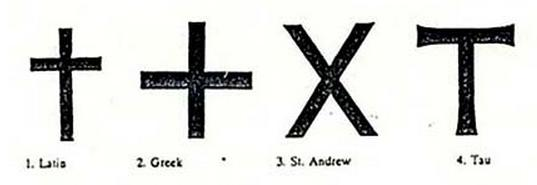
\includegraphics[width=1\textwidth]{cruces.jpg}
    \caption{Distintos tipos de cruces} % URL:http://www.crosses.org/history.htm
\end{figure}

\section{Cristo de San Juan de la Cruz} \label{app:Sanjuan}

\begin{figure}[H]
    \centering
    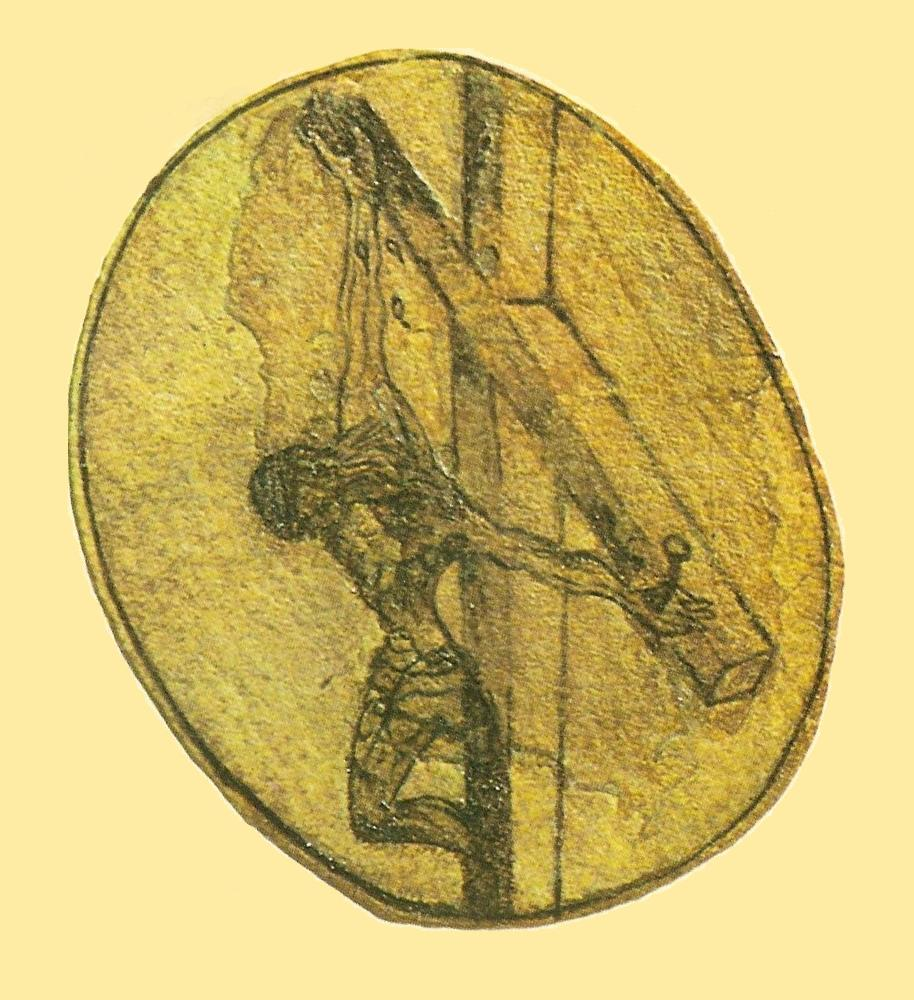
\includegraphics[width=0.55\textwidth]{sanju.jpg}
    \caption{Cristo original de San Juan de la Cruz, que inspiró a Dalí en su obra.} % URL:http://archipielagoduda.blogspot.com.es/2011/03/el-unico-dibujo-conservado-de-san-juan.html
\end{figure}